% This file contains examples of the various styles that can be used in the document.

\lipsum[1]
% \lipsum[1-10]

% This figure will be at the right fixing 13 lines of text
\begin{wrapfigure}[13]{r}{0.41\textwidth}
  \centering
  \includegraphics[width=0.41\textwidth]{../results/qtaim/img/dielsAlder.png}
  \caption{Diels-Alder reaction between itself, the transition state of the dimerisation.}
  \label{diels_alder}
\end{wrapfigure}

\color{blue}
  \begin{quote}
    \textit{... there are several interesting ideas in this paper, but there is one
    you'll never get chemists to believe: the idea that a hydrogen atom can be
    bonded to two other atoms at the same time...}
    \begin{flushright}
      \citet{hildebrand1958wendell}
    \end{flushright}
  \end{quote}
\color{black}

for just units
\SI{}{\kilo \joule \per \mole}

Glossary example
The \gls{IUPAC} defines the HB as follows:

\newpage

% Subfigure
\begin{figure}[h]
  \centering
  \begin{subfigure}[b]{0.43\linewidth}
    \includegraphics[width=\linewidth]{../results/qtaim/img/histogram_carbon_bonds}
    \caption{Differences between carbon bond orders.}
    \label{histogram_carbon}
  \end{subfigure}
  \begin{subfigure}[b]{0.43\linewidth}
    \includegraphics[width=\linewidth]{../results/qtaim/img/histogram_dipole_total}
    \caption{Differences between dipole moments.}
    \label{histogram_dipole}
  \end{subfigure}
  \caption{Caption.}
  \label{fig_coop}
\end{figure}

\dfn{Limit of Sequence}{Let $\{s_n\}$ be a sequence in
We say $$\lim_{n\to\infty}s_n=s$$ where if $\forall$ real numbers
$\varepsilon>0$ $\exists$ natural number $N$ such that for $n>N$
$$s-\varepsilon<s_n<s+\varepsilon\ie |s-s_n|<\varepsilon$$}

\keq{}{Is the set axis a closed set $\rreal$ and $\rreal[n]$ et $\rreal^n$.}

\nt{We will do topology in Normed Linear Space (Mainly $R^n$ and occasionally $C^n$)using the language of Metric Space}

\clm{Topology}{}{Topology is cool}

\cor{}{By the result of the proof, we can then show...}

\thm{}{If $x\in$ open set $V$ then $\exists$ $\delta>0$ such that $B_{\delta}(x)\subset V$}

\mprop{}{$1 + 1 = 2$.}

\begin{myproof} By openness of $V$, $x\in B_r(u)\subset V$
  \begin{center}
    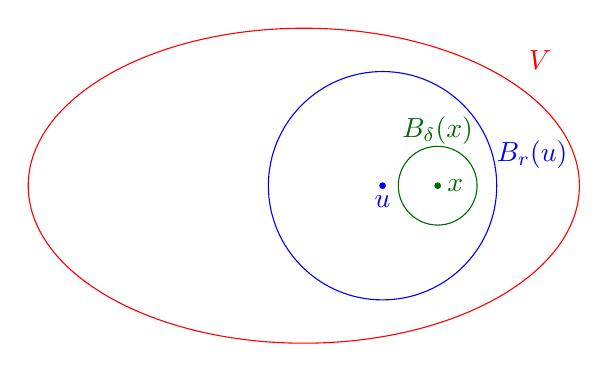
\begin{tikzpicture}
      \draw[red] (0,0) circle [x radius=3.5cm, y radius=2cm] ;
      \draw (3,1.6) node[red]{$V$};
      \draw [blue] (1,0) circle (1.45cm) ;
      \filldraw[blue] (1,0) circle (1pt) node[anchor=north]{$u$};
      \draw (2.9,0.4) node[blue]{$B_r(u)$};
      \draw [green!40!black] (1.7,0) circle (0.5cm) node [yshift=0.7cm]{$B_{\delta}(x)$} ;
      \filldraw[green!40!black] (1.7,0) circle (1pt) node[anchor=west]{$x$};
    \end{tikzpicture}
  \end{center}

  Given $x\in B_r(u)\subset V$, we want $\delta>0$ such that $x\in B_{\delta}
  (x)\subset B_r(u)\subset V$. Let $d=d(u,x)$. Choose $\delta $ such that
  $d+\delta<r$ (e.g. $\delta<\frac{r-d}{2}$)

  If $y\in B_{\delta}(x)$ we will be done by showing that $d(u,y)<r$ but $$d(u,y)\leq d(u,x)+d(x,y)<d+\delta<r$$
\end{myproof}

\begin{tcolorbox}[tab2,tabularx={X||Z|Z|Z|Z||Z}]
Group & One     & Two     & Three    & Four     & Sum      \\\hline\hline
Red   & 1000.00 & 2000.00 &  3000.00 &  4000.00 & 10000.00 \\\hline
Green & 2000.00 & 3000.00 &  4000.00 &  5000.00 & 14000.00 \\\hline
Blue  & 3000.00 & 4000.00 &  5000.00 &  6000.00 & 18000.00 \\\hline\hline
Sum   & 6000.00 & 9000.00 & 12000.00 & 15000.00 & 42000.00
\end{tcolorbox}

\begin{tcolorbox}[tab2,tabularx={X||Z|Z|Z|Z||Z},title=My table,boxrule=0.5pt]
Group & One     & Two     & Three    & Four     & Sum      \\\hline\hline
Red   & 1000.00 & 2000.00 &  3000.00 &  4000.00 & 10000.00 \\
Green & 2000.00 & 3000.00 &  4000.00 &  5000.00 & 14000.00 \\
Blue  & 3000.00 & 4000.00 &  5000.00 &  6000.00 & 18000.00 \\\hline\hline
Sum   & 6000.00 & 9000.00 & 12000.00 & 15000.00 & 42000.00
\end{tcolorbox}

\begin{tcolorbox}[tab1,tabularx={X||ZZZZ||Z}]
Group & One     & Two     & Three    & Four     & Sum      \\\hline\hline
Red   & 1000.00 & 2000.00 &  3000.00 &  4000.00 & 10000.00 \\
Green & 2000.00 & 3000.00 &  4000.00 &  5000.00 & 14000.00 \\
Blue  & 3000.00 & 4000.00 &  5000.00 &  6000.00 & 18000.00 \\\hline\hline
Sum   & 6000.00 & 9000.00 & 12000.00 & 15000.00 & 42000.00
\end{tcolorbox}


Here i go for derivation of the formula for the sum of the first $n$ natural
numbers. Let $S_n=1+2+3+\cdots+n$. Then we have $\Lap$

\begin{align}
  \dv{f}{x} = \lim_{h\to 0} \frac{f(x+h)-f(x)}{h}\\
  \pdv[n]{f}{x} = \lim_{h\to 0} \frac{f(x+h)-f(x)}{h^n}
\end{align}

